\chapter{Árvores Scapegoat}
\chaplabel{scapegoat}

Neste capítulo, estudamos uma estrutura de dados de árvore de busca binária, a #ScapegoatTree#. Essa estrutura é baseada na sabedoria comum de que, quando algo dá errado, a primeira coisa que as pessoas tendem a fazer é encontrar alguém para culpar (o \emph{bode expiatório}).
\index{scapegoat}%
Uma vez que a culpa esteja firmemente estabelecida, podemos deixar o bode expiatório resolver o problema.

Uma #ScapegoatTree# se mantém equilibrada por meio de operações de \emph{reconstrução parcial}.
\index{reconstrução parcial}%
\index{arvore@árvore de busca binária!reconstrução parcial}%
Durante uma operação de reconstrução parcial, uma subárvore inteira é desconstruída e reconstruída em uma subárvore perfeitamente equilibrada. Há muitas maneiras de reconstruir uma subárvore com raiz no nó #u# em uma árvore perfeitamente equilibrada. Um dos mais simples é percorrer a subárvore de #u#, reunindo todos os nós em um array, #a# e, em seguida, criar recursivamente uma subárvore equilibrada usando #a#. Se fizermos $#m#=#a.length#/2$, então o elemento #a[m]# se tornará a raiz da nova subárvore, $#a#[0],\ldots,#a#[#m#-1]$ são armazenados recursivamente na subárvore esquerda e $#a#[#m#+1],\ldots,#a#[#a.length#-1]$ são armazenados recursivamente na subárvore direita.
\codeimport{ods/ScapegoatTree.rebuild(u).packIntoArray(u,a,i).buildBalanced(a,i,ns)}
Uma chamada para #rebuild(u)# leva um tempo $O(#size(u)#)$. A subárvore resultante tem altura mínima; não há árvore de altura menor que tenha #size(u)# nós.

\section{#ScapegoatTree#: Uma Árvore de Busca Binária com Reconstrução Parcial}
\seclabel{scapegoattree}


\index{ScapegoatTree@#ScapegoatTree#}%
Uma #ScapegoatTree# é uma #BinarySearchTree# que, além de rastrear o número #n# dos nós na árvore também mantém um contador, #q#, que mantém um limite superior no número de nós.
\codeimport{ods/ScapegoatTree.q}
Em todos os momentos, #n# e #q# obedecem às seguintes desigualdades:
\[
      #q#/2 \le  #n# \le #q#  \enspace .
\]
Além disso, uma #ScapegoatTree# tem altura logarítmica; nunca a altura da árvore do bode expiatório excede
\begin{equation}
     \log_{3/2} #q# \le \log_{3/2} 2#n# < \log_{3/2} #n# + 2\enspace .
     \eqlabel{scapegoat-height}
\end{equation}
Mesmo com essa restrição, uma #ScapegoatTree# pode parecer surpreendentemente desequilibrada. A árvore em \figref{scapegoat-example} tem $#q#=#n#=10$ e altura $5<\log_{3/2}10 \approx 5.679$.

\begin{figure}
  \begin{center}
    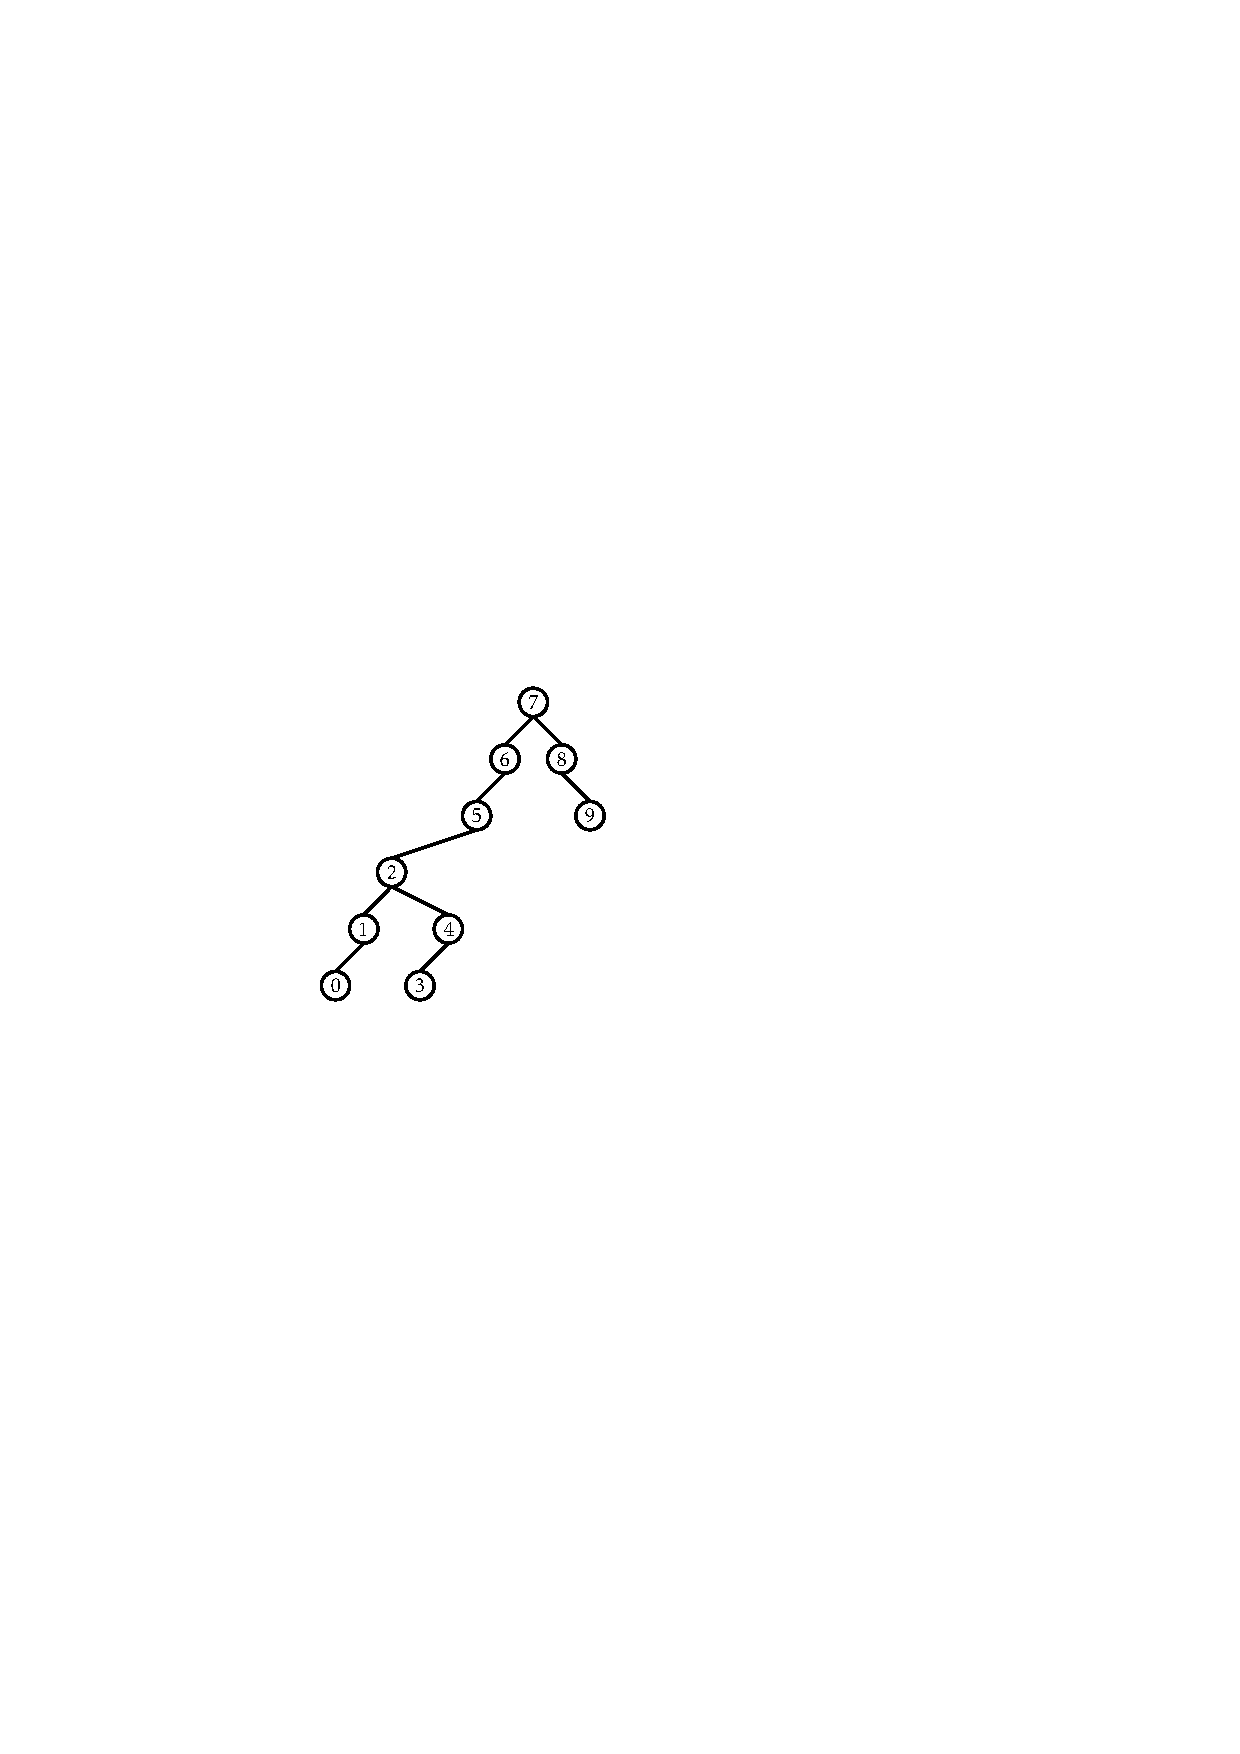
\includegraphics[scale=0.90909]{figs/scapegoat-insert-1}
  \end{center}
  \caption[Uma ScapegoatTree]{Uma #ScapegoatTree# com 10 nós e altura 5.}
  \figlabel{scapegoat-example}
\end{figure}

A implementação da operação #find(x)# em uma #ScapegoatTree# é feita usando o algoritmo padrão para pesquisar em uma #BinarySearchTree# (veja \secref{binarysearchtree}). Isso leva um tempo proporcional à altura da árvore que, por \myeqref{scapegoat-height} é $O(\log #n#)$.

Para implementar a operação #add(x)#, primeiro incrementamos #n# e #q# e usamos o algoritmo usual para adicionar #x# a uma árvore de busca binária; nós procuramos #x# e então adicionamos uma nova folha #u# com $#u.x#=#x#$.
Neste ponto, podemos ter sorte e a profundidade de #u# pode não exceder $\log_{3/2}#q#$. Se assim for, então deixamos como está e não fazemos mais nada.

Infelizmente, às vezes acontece que $#depth(u)# > \log_{3/2}
#q#$. Neste caso, precisamos reduzir a altura. Este não é um grande trabalho; existe apenas um nó, a saber #u#, cuja profundidade excede $\log_{3/2}
#q#$. Para corrigir #u#, percorremos de #u# de volta para a raiz procurando um \emph {bode expiatório}, #w#. O bode expiatório, #w#, é um nó muito desequilibrado. Ele tem a propriedade 
\begin{equation}
   \frac{#size(w.child)#}{#size(w)#} > \frac{2}{3} \enspace ,
   \eqlabel{scapegoat}
\end{equation}
onde #w.child# é o filho de #w# no caminho da raiz para #u#.
Em breve provaremos que existe um bode expiatório. Por enquanto, podemos dar como certo. Uma vez que encontramos o bode expiatório #w#, destruímos completamente a subárvore com raiz em #w# e a reconstruímos em uma árvore de busca binária perfeitamente balanceada. Sabemos, de \myeqref{scapegoat}, que, mesmo antes da adição da subárvore #u#, #w# não era uma árvore binária completa.
Portanto, quando reconstruirmos #w#, a altura diminuirá em pelo menos 1, de modo que a altura da #ScapegoatTree# seja novamente no máximo $\log_{3/2}#q#$.

\codeimport{ods/ScapegoatTree.add(x)}

\begin{figure}
  \begin{center}
    \begin{tabular}{cc}
      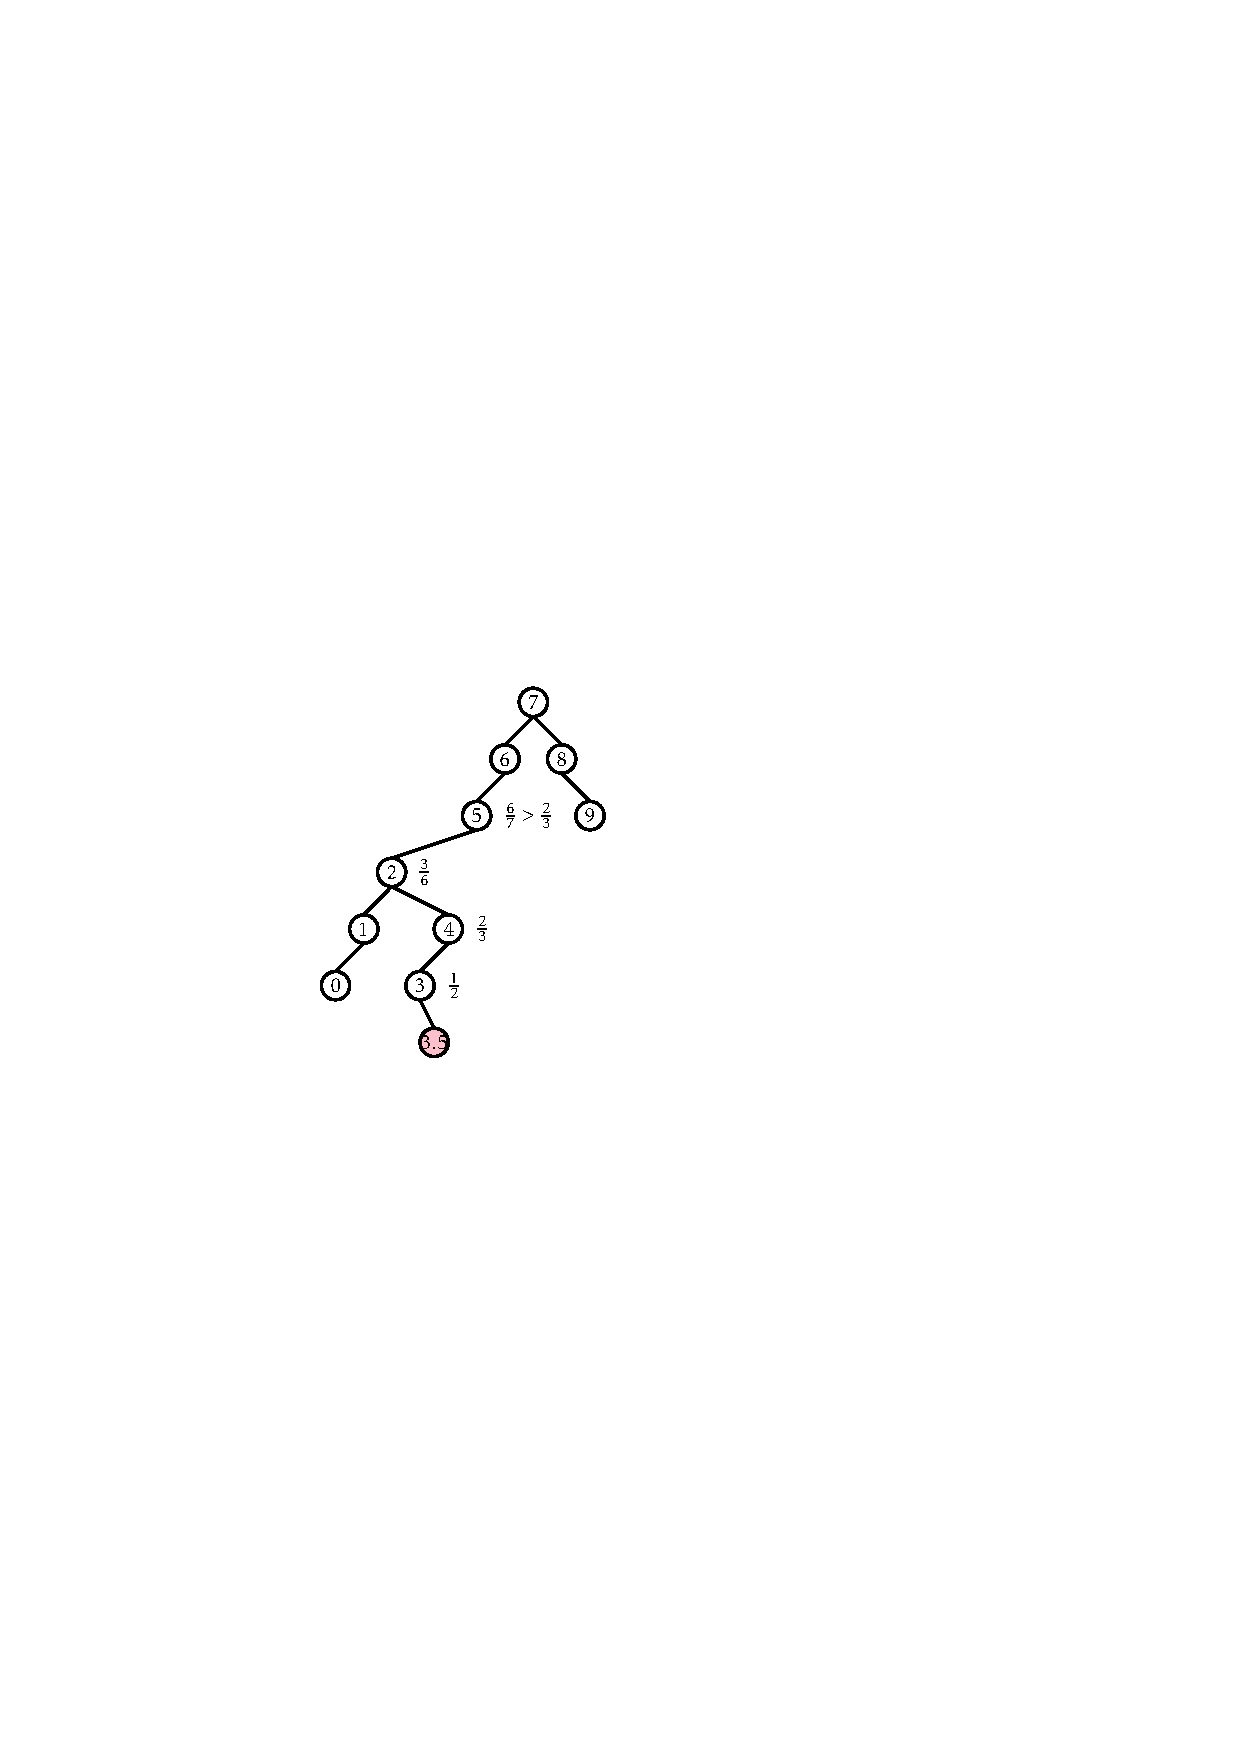
\includegraphics[scale=0.90909]{figs/scapegoat-insert-3} &
      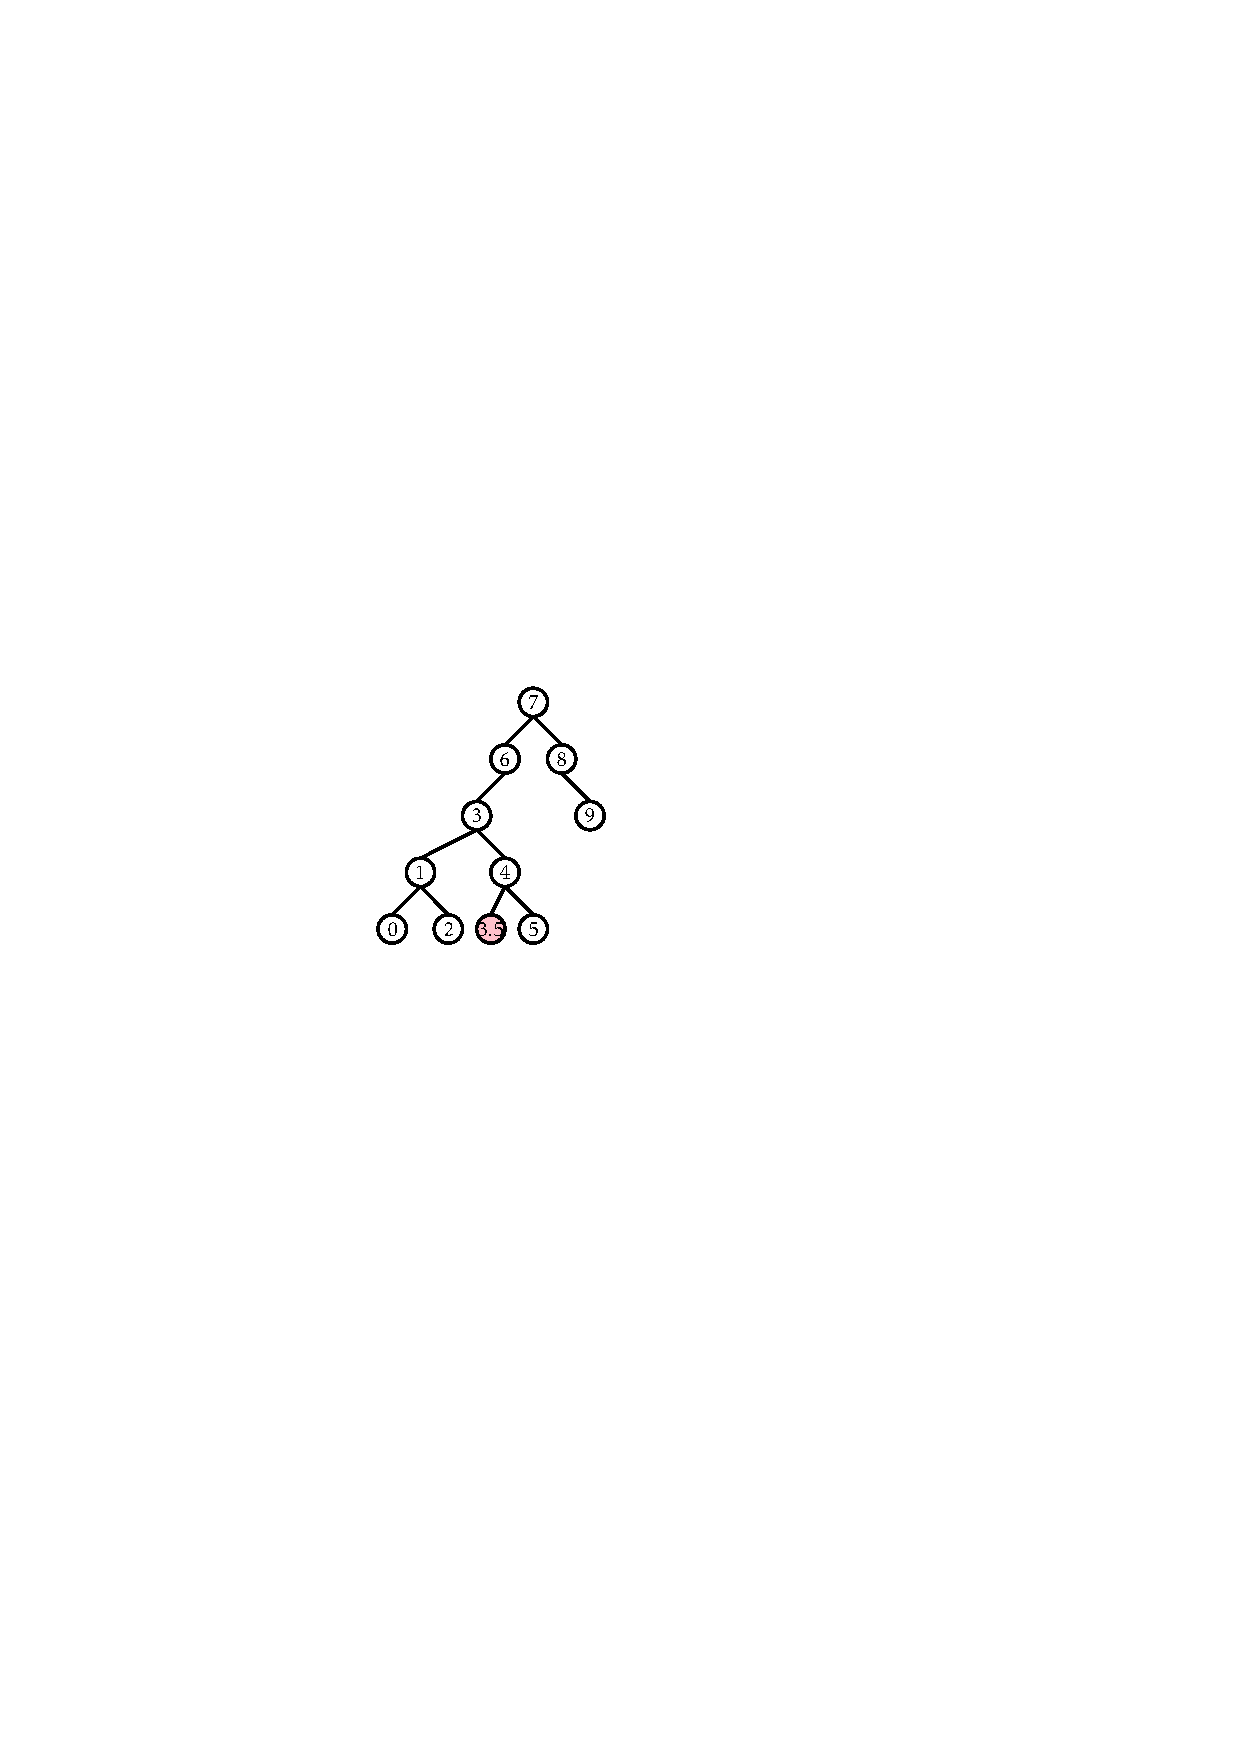
\includegraphics[scale=0.90909]{figs/scapegoat-insert-4} 
    \end{tabular}
  \end{center}
  \caption[Adicionando a uma árvore scapegoat]{Inserindo 3.5 em uma #ScapegoatTree# aumenta sua altura para 6, o que viola \myeqref{scapegoat-height} pois $6 > \log_{3/2} 11 \approx 5.914$.  Um bode expiatório é encontrado no nó contendo 5.}
\end{figure}
Se ignorarmos o custo de encontrar o bode expiatório #w# e reconstruir a
subárvore enraizada em #w#, então o tempo de execução de #add(x)# é dominado pela pesquisa inicial, que toma um tempo $O(\log #q#) = O(\log #n#)$.
Iremos contabilizar o custo de encontrar o bode expiatório e a reconstrução usando a análise amortizada na próxima seção.

A implementação de #remove(x)# em uma #ScapegoatTree# é muito simples.
Nós procuramos #x# e o removemos usando o algoritmo usual para remover um nó de uma #BinarySearchTree#. (Note que isso nunca pode aumentar a altura da árvore). Em seguida, nós decrementamos #n#, mas deixamos #q# inalterado.
Finalmente, nós verificamos se $#q# > 2#n#$ e, em caso afirmativo, então nós \emph{reconstruímos a árvore inteira} em uma árvore de busca binária perfeitamente balanceada e configuramos $#q#=#n#$.
\codeimport{ods/ScapegoatTree.remove(x)}
Novamente, se ignorarmos o custo da reconstrução, o tempo de execução da operação #remove(x)# será proporcional à altura da árvore e, portanto, será $O(\log #n#)$.

\subsection{Análise de Corretude e Tempo de Execução}

Nesta seção, analisamos a corretude e o tempo de execução amortizado das operações em uma #ScapegoatTree#. Primeiro provamos a corretude mostrando que, quando a operação #add(x)# resulta em um nó que viola a Condição \myeqref{scapegoat-height}, então sempre podemos encontrar um bode expiatório:

\begin{lem}
	Seja #u# um nó de profundidade $h>\log_{3/2} #q#$ em uma #ScapegoatTree#. Então existe um nó $#w#$ no caminho do #u# para a raiz tal que
  \[
     \frac{#size(w)#}{#size(parent(w))#} > 2/3 \enspace .
  \]
\end{lem}

\begin{proof}
	Suponha, por uma questão de contradição, que este não é o caso, e
  \[
     \frac{#size(w)#}{#size(parent(w))#} \le 2/3 \enspace .
  \]
  para todos os nós #w# no caminho de #u# para a raiz. Indique o caminho da raiz para #u# como $#r#=#u#_0,\ldots,#u#_h=#u#$. Então nós temos
  $#size(u#_0#)#=#n#$,
  $#size(u#_1#)#\le\frac{2}{3}#n#$, 
  $#size(u#_2#)#\le\frac{4}{9}#n#$ e, de maneira mais geral,
  \[
  #size(u#_i#)#\le\left(\frac{2}{3}\right)^i#n# \enspace .
  \]
  Mas isso gera uma contradição, já que $#size(u)#\ge 1$, daí
  \[
    1 \le #size(u)# \le \left(\frac{2}{3}\right)^h#n#
   < \left(\frac{2}{3}\right)^{\log_{3/2} #q#}#n#
   \le \left(\frac{2}{3}\right)^{\log_{3/2} #n#}#n#
   = \left(\frac{1}{#n#}\right) #n#
   = 1 \enspace . \qedhere
  \]
\end{proof}

Em seguida, analisamos as partes do tempo de execução que ainda não foram contabilizadas. Existem duas partes: o custo das chamadas para #size(u)# ao procurar por nós de bodes expiatórios e o custo das chamadas para #rebuild(w)# quando encontramos um bode expiatório #w#. O custo das chamadas para #size(u)# pode estar relacionado ao custo das chamadas para #rebuild(w)#, da seguinte forma:
\begin{lem}
	Durante uma chamada para #add(x)# em uma #ScapegoatTree#, o custo de encontrar o bode expiatório #w# e reconstruir a subárvore com raiz em #w# é $O(#size(w)#)$.
\end{lem}

\begin{proof}
	O custo de reconstruir o nó do bode expiatório #w#, uma vez encontrado, é $O(#size(w)#)$. Ao procurar pelo nó do bode expiatório, chamamos #size(u)#
	em uma sequência de nós $#u#_0,\ldots,#u#_k$ até encontrarmos o bode expiatório $#u#_k=#w#$. No entanto, como $#u#_k$ é o primeiro nó dessa sequência que é um bode expiatório, sabemos que
\[
  #size(u#_{i}#)# < \frac{2}{3}#size(u#_{i+1}#)#
\]
para todo $i\in\{0,\ldots,k-2\}$.  Portanto, o custo de todas as chamadas para #size(u)# é
\begin{eqnarray*}
 O\left( \sum_{i=0}^k #size(u#_{k-i}#)# \right)
 &=& O\left(
  #size(u#_k#)# 
  + \sum_{i=0}^{k-1} #size(u#_{k-i-1}#)#
  \right) \\
 &=& O\left(
  #size(u#_k#)# 
  + \sum_{i=0}^{k-1} \left(\frac{2}{3}\right)^i#size(u#_{k}#)#
  \right) \\
&=& O\left(
  #size(u#_k#)#\left(1+ 
   \sum_{i=0}^{k-1} \left(\frac{2}{3}\right)^i
  \right)\right) \\
&=& O(#size(u#_k#)#) = O(#size(w)#) \enspace ,
\end{eqnarray*}
onde a última linha segue do fato de que a soma é uma série geometricamente decrescente.
\end{proof}

Tudo o que resta é provar um limite superior no custo de todas as chamadas para #rebuild(u)# durante uma sequência de $m$ operações:

\begin{lem}\lemlabel{scapegoat-amortized}
	Começando com uma #ScapegoatTree# vazia, qualquer sequência de $m$ operações #add(x)# e #remove(x)# causam um tempo de no máximo $O(m\log m)$ a ser usado pelas operações de #rebuild(u)#.
\end{lem}

\begin{proof}
	Para provar isso, usaremos um \emph {esquema de crédito}.
  \index{esquema de crédito}%
  Nós imaginamos que cada nó armazena um número de créditos. Cada crédito pode pagar por algumas unidades de tempo gasto $c$ constante na reconstrução. O esquema dá um total de $O(m\log m)$ créditos e cada chamada para #rebuild (u) # é paga com créditos armazenados em #u#.

  Durante uma inserção ou exclusão, damos um crédito a cada nó no caminho para o nó inserido ou nó excluído, #u#. Desta forma distribuímos no máximo $\log_{3/2}#q#\le \log_{3/2}m$ créditos por operação.
  Durante uma exclusão, também armazenamos um crédito adicional ``de lado''.
  Assim, no total, distribuímos no máximo $O(m\log m)$ créditos. Tudo o que resta é mostrar que esses créditos são suficientes para pagar todas as chamadas para #rebuild(u)#.

  Se chamarmos #rebuild(u)# durante uma inserção, é porque #u# é um bode expiatório. Suponha, sem perda de generalidade, que
  \[
    \frac{#size(u.left)#}{#size(u)#} > \frac{2}{3} \enspace .
  \]
  Usando o fato que
  \[
    #size(u)# = 1 + #size(u.left)# + #size(u.right)# 
  \]
  deduzimos que
  \[
    \frac{1}{2}#size(u.left)# > #size(u.right)#  \enspace 
  \]
  e, portanto,
  \[
    #size(u.left)# - #size(u.right)# > \frac{1}{2}#size(u.left)# >
    \frac{1}{3}#size(u)#  \enspace .
  \]
  Agora, a última vez que uma subárvore contendo #u# foi reconstruída (ou quando #u# foi inserido, se uma subárvore contendo #u# nunca foi reconstruída), temos
  \[
    #size(u.left)# - #size(u.right)# \le 1 \enspace .
  \]
  Portanto, o número de operações #add(x)# ou #remove(x)# que afetaram #u.left# ou #u.right# desde então é pelo menos
  \[
    \frac{1}{3}#size(u)# - 1 \enspace . 
  \]
  e há, portanto, pelo menos, tantos créditos armazenados em #u# que estão disponíveis para pagar pelo tempo $O(#size(u)#)$ que leva para chamar #rebuild(u)#.

  Se chamarmos #rebuild(u)# durante uma exclusão, é porque $#q# > 2#n#$.
  Neste caso, temos $#q#-#n#> #n#$ créditos armazenados ``de lado'', e nós os usamos para pagar o tempo $O(#n#)$ que leva para reconstruir a raiz.
  Isso conclui a prova.
\end{proof}

\subsection{Resumo}
O seguinte teorema resume o desempenho da estrutura de dados #ScapegoatTree#:

\begin{thm}\thmlabel{scapegoat}
  Uma #ScapegoatTree# implementa a interface #SSet#. Ignorando o custo das operações de #rebuild(u)#, uma #ScapegoatTree# suporta as operações #add(x)#, #remove(x)# e #find(x)# em tempo $O(\log #n#)$ por operação.
  
  Além disso, começando com uma #ScapegoatTree# vazia, qualquer sequência de $m$ operações #add(x)# e #remove(x)#  resulta em um total de $O(m\log m)$ de tempo gasto durante todas as chamadas para #rebuild(u)#.
\end{thm}

\section{Discussão e Exercícios}

O termo \emph {árvore scapegoat} é creditado a Galperin e Rivest \cite{gr93}, que definem e analisam essas árvores. No entanto, a mesma estrutura foi descoberta anteriormente por Andersson \cite{a89, a99}, que as chamou de \emph{árvores balanceadas geral}, 
\index{arvore@árvore balanceada geral}%
já que elas podem ter qualquer forma desde que sua altura seja pequena.

Teste experimentais com a implementação da #ScapegoatTree# revelará que ela é consideravelmente mais lenta que as outras implementações de #SSet# neste livro. Isso pode ser um pouco surpreendente, já que a altura limitada a
\[
   \log_{3/2}#q# \approx 1.709\log #n# + O(1)
\] 
é melhor que o tamanho esperado de um caminho de busca em uma #Skiplist# e não muito distante de uma #Treap#. A implementação pode ser otimizada armazenando os tamanhos de subárvores explicitamente em cada nó ou reutilizando os tamanhos de subárvores já calculados (Exercícios~\ref{exc:scapegoat-quicksize} e \ref{exc:scapegoat-explicitsize}). Mesmo com essas otimizações, sempre haverá sequências de operações #add(x)# e #delete(x)# para as quais a #ScapegoatTree# demora mais que outras implementações de #SSet#.

Essa lacuna no desempenho se deve ao fato de que, diferentemente das outras implementações da #SSet# discutidas neste livro, uma #ScapegoatTree# pode passar muito tempo se reestruturando. \excref{scapegoat-nlogn} pede para você provar que existem sequências de #n# operações nas quais a #ScapegoatTree# irá gastar um tempo da ordem de $#n#\log #n#$ em chamadas para #rebuild(u)#.
Isso está em contraste com outras implementações do #SSet# discutidas neste livro, que fazem apenas $O(#n#)$ alterações estruturais durante uma sequência de #n# operações. Esta é, infelizmente, uma consequência necessária do fato de que uma #ScapegoatTree# faz toda a sua reestruturação por meio de chamadas para #rebuild(u)# \cite{d90}.

Apesar de sua falta de desempenho, existem aplicações em que uma #ScapegoatTree# poderia ser a escolha certa. Isso ocorreria sempre que houvesse dados adicionais associados a nós que não pudessem ser atualizados em tempo constante quando uma rotação fosse executada, mas que pudesse ser atualizada durante uma operação de #rebuild(u)#. Em tais casos, a #ScapegoatTree# e estruturas relacionadas baseadas em reconstrução parcial podem funcionar. Um exemplo de tal aplicação é descrito em \excref{list-order-maintenance}.

\begin{exc}
	Ilustre a adição dos valores 1.5 e 1.6 na #ScapegoatTree# em \figref{scapegoat-example}.
\end{exc}

\begin{exc}
	Ilustre o que acontece quando a sequência $1,5,2,4,3$ é adicionada a uma #ScapegoatTree# vazia e mostre onde os créditos descritos na prova do \lemref{scapegoat-amortized} vão e como eles são usados durante essa sequência de adições.
\end{exc}

\begin{exc}\exclabel{scapegoat-nlogn}
	Mostre que, se começarmos com uma #ScapegoatTree# vazia e chamarmos #add(x)# para $#x#=1,2,3,\ldots,#n#$, então o tempo total gasto durante as chamadas para #rebuild(u)# é de pelo menos $c#n#\log #n#$ para alguma constante $c>0$.
\end{exc}

\begin{exc}
	A #ScapegoatTree#, conforme descrita neste capítulo, garante que o comprimento do caminho de pesquisa não exceda $\log_{3/2}#q#$.
  \begin{enumerate}
    \item  Projete, analise e implemente uma versão modificada de #ScapegoatTree# onde o comprimento do caminho de pesquisa não exceda $\log_{#b#} #q#$, onde #b# é um parâmetro com $1<#b#<2$.
    \item O que sua análise e/ou seus experimentos dizem sobre o custo amortizado de #find(x)#, #add(x)# e #remove(x)# como uma função de #n# e #b#?
  \end{enumerate}
\end{exc}

\begin{exc}\exclabel{scapegoat-quicksize}
	Modifique o método #add(x)#  da #ScapegoatTree# para que ele não perca tempo recalculando os tamanhos de subárvores que já foram computados. Isso é possível porque, no momento em que o método deseja calcular #size(w)#, ele já calculou um dos #size(w.left)# ou #size(w.right)#. Compare o desempenho de sua implementação modificada com a implementação fornecida aqui.
\end{exc}

\begin{exc}\exclabel{scapegoat-explicitsize}
	Implemente uma segunda versão da estrutura de dados #ScapegoatTree# que armazena e mantém explicitamente os tamanhos da subárvore com raiz em cada nó. Compare o desempenho da implementação resultante com a implementação original de #ScapegoatTree#, bem como a implementação de \excref{scapegoat-quicksize}.
\end{exc}

\begin{exc}
	Reimplemente o método #rebuild(u)# discutido no início deste capítulo para que ele não exija o uso de um array para armazenar os nós da subárvore que está sendo reconstruída. Em vez disso, ele deve usar recursão para primeiro conectar os nós a uma lista encadeada e depois converter essa lista encadeada em uma árvore binária perfeitamente balanceada. (Existem implementações recursivas muito elegantes de ambas as etapas.)
\end{exc}

\begin{exc}
  \index{WeightBalancedTree@#WeightBalancedTree#}%
  Analise e implemente uma #WeightBalancedTree#. Esta é uma árvore na qual cada nó #u#, exceto a raiz, mantém o \emph {invariante de equilíbrio} no qual $#size(u)# \le (2/3)#size(u.parent)#$. As operações #add(x)# e #remove(x)# são idênticas às operações da #BinarySearchTree# padrão, exceto que sempre que a invariante de balanceamento for violada em um nó #u#, a subárvore com raiz em #u.parent# é reconstruída.
  Sua análise deve mostrar que as operações na #WeightBalancedTree# são executadas em um tempo amortizado de $O(\log#n#)$.
\end{exc}

\begin{exc}
  \index{CountdownTree@#CountdownTree#}%
  Analise e implemente uma #CountdownTree#. Em uma #CountdownTree#, cada nó #u# mantém um \emph{temporizador} #u.t#. As operações #add(x)# e #remove(x)# são exatamente as mesmas que em uma #BinarySearchTree# padrão, exceto que, sempre que uma dessas operações afeta a subárvore #u#, #u.t# é decrementado. Quando $#u.t#=0$, toda a subárvore com raiz em #u# é reconstruída em uma árvore de busca binária perfeitamente balanceada. Quando um nó #u# está envolvido em uma operação de reconstrução (seja porque #u# foi recriado ou um dos ancestrais de #u# foi reconstruído) #u.t# é reiniciado para $#size(u)#/3$.

  Sua análise deve mostrar que as operações em uma #CountdownTree# são executadas em um tempo amortizado de $O(\log #n#)$. (Dica: primeiro mostre que cada nó #u# satisfaz a alguma versão de uma invariante de balanceamento.)
\end{exc}

\begin{exc}
  \index{DynamiteTree@#DynamiteTree#}%
  Analise e implemente uma #DynamiteTree#. Em uma #DynamiteTree#, cada nó #u# mantém as informações sobre o tamanho da subárvore com raiz em #u# em uma variável #u.size#. As operações #add(x)# e #remove(x)# são exatamente as mesmas que em uma #BinarySearchTree# padrão, exceto que, sempre que uma dessas operações afetar uma subárvore do nó #u#, #u# \emph{explode} com probabilidade $1/#u.size#$. Quando #u# explode, toda a subárvore é reconstruída em uma árvore de busca binária perfeitamente balanceada.

  Sua análise deve mostrar que as operações em uma #DynamiteTree# são executadas em um tempo esperado igual a $O(\log #n#)$.
\end{exc}
 

\begin{exc}\exclabel{list-order-maintenance}
  \index{Sequencia@#Sequencia#}%
  Projete e implemente uma estrutura de dados #Sequencia# que mantenha uma sequência (lista) de elementos. Ela suporta estas operações:
  \begin{itemize}
    \item #addAfter(e)#: Adiciona um novo elemento após o elemento #e# na sequência. Retorna o elemento recém-adicionado. (Se #e# for nulo, o novo elemento será adicionado no início da sequência.)
    \item #remove(e)#: Remove #e# da sequencia.
    \item #testBefore(e1,e2)#: retorna #true# se e somente se #e1# venha antes de #e2# na sequência.
  \end{itemize}
  As duas primeiras operações devem ser executadas em um tempo amortizado igual a $O(\log #n#)$.
  A terceira operação deve ser executada em tempo constante.

  A estrutura de dados #Sequence# pode ser implementada ao armazenar os elementos em algo como uma #ScapegoatTree#, na mesma ordem em que ocorrem na sequência. Para implementar #testBefore(e1,e2)# em tempo constante, cada elemento #e# é rotulado com um inteiro que codifica o caminho da raiz para #e#. Dessa forma, #testBefore(e1,e2)# pode ser implementado comparando os rótulos de #e1# e #e2#.
\end{exc}

